% ╭──────────────────────────────────────────────────────────╮
% │                 Road to BV Quantization                  │
% ╰──────────────────────────────────────────────────────────╯
\documentclass{standalone}

\usepackage{tikz}
\usetikzlibrary{cd}

\begin{document}
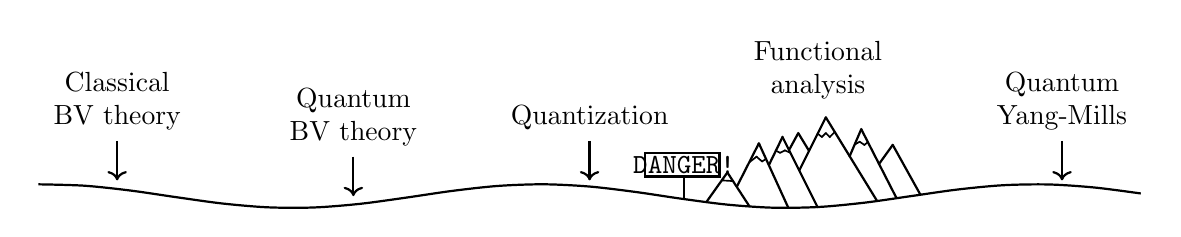
\begin{tikzpicture}
  \draw[thick, domain=-7:7, smooth, variable=\x] plot ( {\x}, {0.15*sin(deg(\x+2.2))} );
  \node at (-6, 1.2) {
    \begin{tabular}{c}
      Classical \\
      BV theory
    \end{tabular}
  };
  \draw[thick, ->] (-6, .7) -- (-6, .2);
  \node at (-3, 1) {
    \begin{tabular}{c}
      Quantum \\
      BV theory
    \end{tabular}
  };
  \draw[thick, ->] (-3, .5) -- (-3, 0);
  \node at (0, 1) { Quantization };
  \draw[thick, ->] (0, .7) -- (0, .2);
  \node at (2.9, 1.6) {
    \begin{tabular}{c}
      Functional \\
      analysis
    \end{tabular}
  };
  \node at (1.2, .4) { \miniscule\texttt{DANGER!} };
  \draw[thick] (.7, .25) rectangle ++(.95, .3);
  \draw[thick] (1.2, .25) -- (1.2, -.03);
  \node at (6, 1.2) {
    \begin{tabular}{c}
      Quantum \\ 
      Yang-Mills
    \end{tabular}
  };
  \draw[thick, ->] (6, .7) -- (6, .2);
% ── Mountains ─────────────────────────────────────────────────────────
  \draw[thick] (1.48, -.08) -- (1.75, 0.3);
  \draw[thick] (1.75, 0.3) -- (2.03, -.13);
  \draw[fill] (1.75, 0.3) circle (.2pt);
  \draw[semithick] (1.67, .2) -- (1.83, 0.19);
  \draw[thick] (1.87, .12) -- (2.15, 0.67);
  \draw[thick] (2.15, 0.67) -- (2.52, -.14);
  \draw[fill] (2.15, 0.67) circle (.19pt);
  \draw[semithick] (2.03, 0.43) -- (2.12, 0.5);
  \draw[fill] (2.12, 0.5) circle (.101pt);
  \draw[semithick] (2.12, 0.5) -- (2.19, 0.44);
  \draw[fill] (2.19, 0.44) circle (.101pt);
  \draw[semithick] (2.19, 0.44) -- (2.24, 0.47);
  \draw[thick] (2.28, .4) -- (2.45, 0.75);
  \draw[thick] (2.45, 0.75) -- (2.9, -.15);
  \draw[fill] (2.45, 0.75) circle (.19pt);
  \draw[semithick] (2.36, 0.58) -- (2.42, 0.55);
  \draw[fill] (2.42, 0.55) circle (.101pt);
  \draw[semithick] (2.42, 0.55) -- (2.48, 0.58);
  \draw[fill] (2.48, 0.58) circle (.101pt);
  \draw[semithick] (2.48, 0.58) -- (2.55, 0.55);
  \draw[thick] (2.53, .58) -- (2.65, 0.8);
  \draw[thick] (2.65, 0.8) -- (2.79, .57);
  \draw[fill] (2.65, 0.8) circle (.19pt);
  \draw[thick] (2.66, .32) -- (3, 1);
  \draw[thick] (3.65, -.06) -- (3, 1);
  \draw[fill] (3, 1) circle (.19pt);
  \draw[semithick] (2.89, .8) -- (2.95, .75);
  \draw[fill] (2.95, 0.75) circle (.101pt);
  \draw[semithick] (2.95, .75) -- (3, .8);
  \draw[fill] (3, 0.8) circle (.101pt);
  \draw[semithick] (3, .8) -- (3.05, 0.75);
  \draw[fill] (3.05, 0.75) circle (.101pt);
  \draw[semithick] (3.05, 0.75) -- (3.12, 0.82);
  \draw[thick] (3.3, 0.5) -- (3.45, 0.85);
  \draw[thick] (3.45, 0.85) -- (3.9, -.03);
  \draw[fill] (3.45, 0.85) circle (0.19pt);
  \draw[semithick] (3.36, .65) -- (3.43, .69);
  \draw[fill] (3.43, .69) circle (.101pt);
  \draw[semithick] (3.43, .69) -- (3.49, .65);
  \draw[fill] (3.49, .65) circle (.101pt);
  \draw[semithick] (3.49, .65) -- (3.54, .69);
  \draw[thick] (3.67, .4) -- (3.85, .65);
  \draw[thick] (3.85, 0.65) -- (4.2, 0.02);
  \draw[fill] (3.85, 0.65) circle (.19pt);
\end{tikzpicture}
\end{document}

